\chapter*{Dodatak: Prikaz aktivnosti grupe}
		\addcontentsline{toc}{chapter}{Dodatak: Prikaz aktivnosti grupe}

		\section*{Dnevnik sastajanja}

		\begin{packed_enum}
			\item  sastanak
			\item[] \begin{packed_item}
				\item Datum: 14. listopada 2022.
				\item Prisustvovali: Svi članovi
				\item Teme sastanka:
				\begin{packed_item}
					\item  upoznavanje članova
					\item  raspravljanje o podjeli posla
					\item  inicijalni "brainstorming"
				\end{packed_item}
			\end{packed_item}

			\item  sastanak
			\item[] \begin{packed_item}
				\item Datum: 23. listopada 2022.
				\item Prisustvovali: Svi članovi
				\item Teme sastanka:
				\begin{packed_item}
					\item  inicijalni oblik baze podataka
					\item  razrađivanje projektnog zadatka
				\end{packed_item}
			\end{packed_item}

			\item  sastanak
			\item[] \begin{packed_item}
				\item Datum: 30. listopada 2022.
				\item Prisustvovali: Svi članovi
				\item Teme sastanka:
				\begin{packed_item}
					\item  raspored posla do idućeg sastanka
					\item  dizajn ekrana aplikacije - funkcionalost i \textit{Frontend} dizajn
				\end{packed_item}
			\end{packed_item}

			\item  sastanak
			\item[] \begin{packed_item}
				\item Datum: 08. studenog 2022.
				\item Prisustvovali: Svi članovi
				\item Teme sastanka:
				\begin{packed_item}
					\item  raspored posla do "laboratorijske vježbe" demonstracije do sad napravljenog posla.
				\end{packed_item}
			\end{packed_item}

			\item  sastanak
			\item[] \begin{packed_item}
				\item Datum: 15. studenog 2022.
				\item Prisustvovali: Svi članovi
				\item Teme sastanka:
				\begin{packed_item}
					\item  pregled do sada napravljenog posla i preostalog posla
					\item raspodjela posla do predaje projekta za kraj 1. ciklusa nastave
				\end{packed_item}
			\end{packed_item}

                \item  sastanak
			\item[] \begin{packed_item}
				\item Datum: 10. prosinca 2022.
				\item Prisustvovali: Svi članovi
				\item Teme sastanka:
				\begin{packed_item}
					\item  pregled i raspodjela glavnog posla za 2. ciklus
					\item  druženje unutar tima pomoću aplikacije Discord
				\end{packed_item}
			\end{packed_item}

                \item  sastanak
			\item[] \begin{packed_item}
				\item Datum: 10. siječnja 2022.
				\item Prisustvovali: Svi članovi
				\item Teme sastanka:
				\begin{packed_item}
					\item  pregled napravljenog posla pred predaju
				\end{packed_item}
			\end{packed_item}

			%

		\end{packed_enum}

		\eject
		\section*{Tablica aktivnosti}


			\begin{longtblr}[
					label=none,
				]{
					vlines,hlines,
					width = \textwidth,
					colspec={X[7, l]X[1, c]X[1, c]X[1, c]X[1, c]X[1, c]X[1, c]X[1, c]},
					vline{1} = {1}{text=\clap{}},
					hline{1} = {1}{text=\clap{}},
					rowhead = 1,
				}
				\multicolumn{1}{c|}{} & \multicolumn{1}{c|}{\rotatebox{90}{\textbf{Ian Golob}}} & \multicolumn{1}{c|}{\rotatebox{90}{\textbf{Matej Košćec }}} &	\multicolumn{1}{c|}{\rotatebox{90}{\textbf{Edi Prodan }}} & \multicolumn{1}{c|}{\rotatebox{90}{\textbf{Zvonimir Žunić }}} &	\multicolumn{1}{c|}{\rotatebox{90}{\textbf{Josip Goluža }}} & \multicolumn{1}{c|}{\rotatebox{90}{\textbf{Adrian Sušec }}} &	\multicolumn{1}{c|}{\rotatebox{90}{\textbf{Ivan Kolar }}} \\
				Upravljanje projektom 		& 4 &  &  &  & &  & \\
				Opis projektnog zadatka 	&  &  &  &  &  & & 2 \\

				Funkcionalni zahtjevi       &  &  &  &  &  & & 2  \\
				Opis pojedinih obrazaca 	&  &  &  &  &  & & 6  \\
				Dijagram obrazaca 			&  &  &  &  &  & & 2  \\
				Sekvencijski dijagrami 		&  &  &  &  &  & & 6  \\
				Opis ostalih zahtjeva 		&  &  &  &  &  & & 1  \\

				Arhitektura i dizajn sustava	 &  &  &  &  & & & 5    \\
				Baza podataka				 & 10  &  &  &  & & & 4   \\
				Dijagram razreda 			 & 3  &  &  &  & & & 1   \\
				Dijagram stanja				&  &  &  &  &  & & 2&   \\
				Dijagram aktivnosti 		&  &  &  &  &  & & 2&  \\
				Dijagram komponenti			&  &  &  &  &  & & 2&  \\
				Korištene tehnologije i alati 		 & 1 & 0.5 & &  &  &  & 2 \\
				Ispitivanje programskog rješenja 	& 12 &  & & &  &  &  &  \\
				Dijagram razmještaja			&  &  &  & & &  & 1 &  \\
				Upute za puštanje u pogon 		&  & 1 &  & & &  &  &  \\
				Dnevnik sastajanja 			&  &  &  &  & & 2 &   \\
				Zaključak i budući rad 		&  &  &  &  & & & 2 &  \\
				Popis literature 			&  &  &  &  & & & 0.5 & \\
				&  &  &  &  &  &  &  \\ \hline
				Izrada baze podataka		 			 & 2 & 1 &  &  &  & \\
				Spajanje s bazom podataka 							& 0.5  &  &  &  &  &  &  \\
				Dizajn stranice 							& 5 & 15  &  10 & 3 &  & 8 & \\
				\textit{Backend} 							 & 58 & 65  & 20 & 9 & 26 & 35 & \\
				\textit{Frontend} 							 & 5 & 60  & 55 & 50 & 40 & 50 & \\
				Puštanje aplikacije u pogon     &  & 25  &  &  &  &  &  & \\
			\end{longtblr}


		\eject

		\section*{Dijagrami pregleda promjena}

		%\textbf{\textit{dio 2. revizije}}\\

		%\textit{Prenijeti dijagram pregleda promjena nad datotekama projekta. Potrebno je na kraju projekta generirane grafove s gitlaba prenijeti u ovo poglavlje dokumentacije. Dijagrami za vlastiti projekt se mogu preuzeti s gitlab.com stranice, u izborniku Repository, pritiskom na stavku Contributors.}
		                  \begin{figure}[H]
                			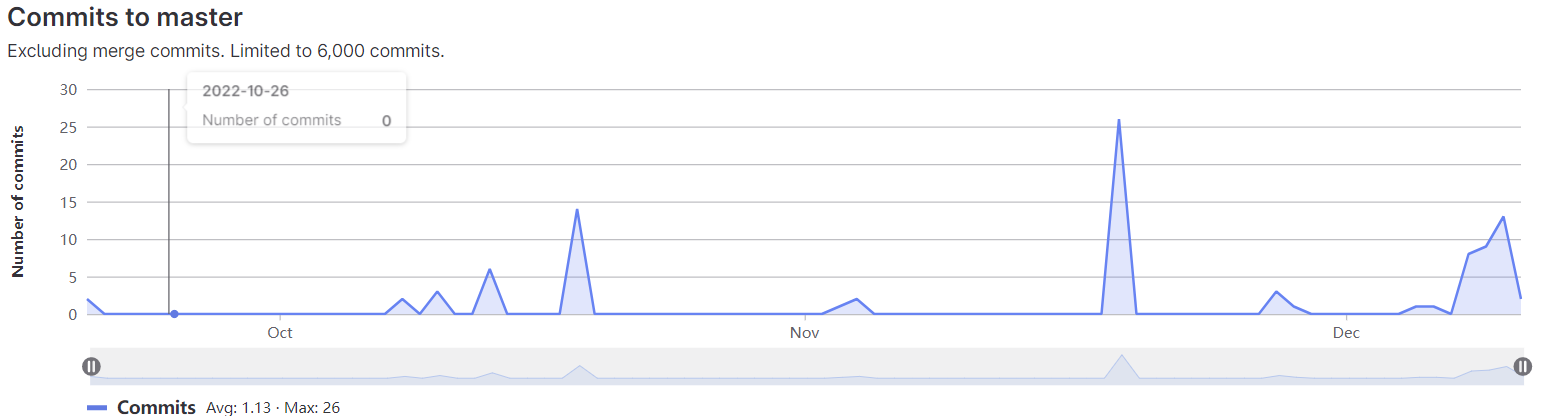
\includegraphics[scale=0.4]{slike/backend_master.PNG} %veličina slike u odnosu na originalnu datoteku i pozicija slike
                			\centering
                			\caption{Pregled promjena - \textit{backend}}
                			
                		\end{figure}

                            \begin{figure}[H]
                			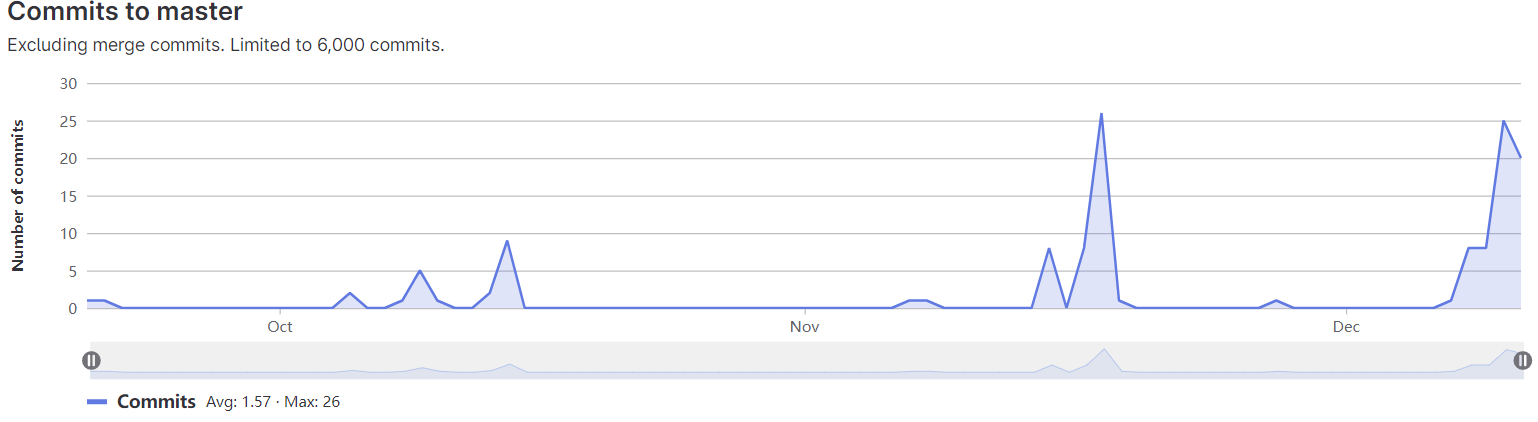
\includegraphics[scale=0.4]{slike/front_master.PNG} %veličina slike u odnosu na originalnu datoteku i pozicija slike
                			\centering
                			\caption{Pregled promjena - \textit{frontend}}
                			
                		\end{figure}
	